\documentclass{article}
\usepackage{graphicx}
\usepackage{hyperref}
\usepackage{color}

\begin{document}

\title{Poppy software quickstart guide}
\author{Manon Cortial, Generation Robots}

\maketitle

  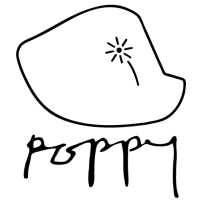
\includegraphics[height=0.22\textwidth]{img/poppy-logo} \hfill 
\includegraphics[height=0.22\textwidth]{img/GR-logo}

\section{Introduction}

\subsection{The Poppy Project}

Poppy is an open hardware and open-source project, containing in particular the Poppy Humanoid robot. The library that was created by the Liris to control the robot is named Pypot. It is in constant evolution, thanks to the engineers of Liris and to the community, so keep posted.

%The programmation in made essentially in Python, but it is also possible to control the robot with visual programming using Snap!.

%All links to the forum and online documentations are grouped in the section \ref{documentation-links}.

\subsection{How to use this guide?}

This guide gives you an introduction to Poppy programming and helps you to set up your system and find the relevant documentations and tutorial in the Poppy environment.

If you are a \textbf{Poppy user} (beginner, teacher, artist...), you will mostly use the webserver (section \ref{poppy-webservices}) and Snap! (section \ref{programming-with-snap}).

If you are a \textbf{Poppy developper} (student, researcher, application developper...), you want to know about the webserver (section \ref{poppy-webservices}) and the pypot library (section \ref{pypot})

If you \textbf{don't have a Poppy robot}, see section \ref{installing-pypot} to setup your computer, section \ref{v-rep} for the V-REP simulator, then have a look at Snap! (section \ref{programming-with-snap}) or Pypot (section \ref{pypot}).

If you are a \textbf{Poppy contributor}, you want to know about it all! ;-)

\subsection{\textcolor{red}{Safety warning}}

The Poppy humanoid robot is built using mainly MX-28 Dynamixel servomotors, which are pretty powerful and may be harmful to your fingers or materials.

So be very careful and put the robot in a free space while testing your programs.

\subsection{Useful tools}

\subsubsection{Bonjour}

Bonjour is a software made by the Apple company to communicate with a device using its name instead of its IP address.

It is installed by default on Mac and most Linux. Windows users can find an installer here: \url{https://support.apple.com/kb/DL999?locale=fr_FR&viewlocale=fr_FR}

If you don't want to use Bonjour, replace all occurences of 'poppy.local' by the IP address of the robot in this tutorial.

\subsubsection{SSH}

SSH means Secure SHell. It's a protocol allowing to open a terminal from another device (say, your robot) on your computer.

We will use SSH to have a look at the documents in the robot, change the settings and install new programs. If you are only using the webservices and/or Snap!, you don't need SSH.

SSH is installed by default on Mac and most Linux. The most popular SSH software for Windows is \href{http://www.putty.org/}{Putty}.

\subsubsection{Git and Github}

Git is a versioning software, very useful to secure older versions of your code while workig on a new one. It also allows to merge different modifications from different developpers on the same project.

Github is a website offering free remote hosting for Git project (if they are public). All sources for Poppy are on \href{https://github.com/poppy-project}{Github}.

Git is not installed by default. For Debian and Fedora based computer, the packet is called git. For Mac, have a look at \url{http://sourceforge.net/projects/git-osx-installer/}. For Windows, find the installer here: \url{http://msysgit.github.io/}.

If you are mainly a user, you will use \textit{git clone} to get new packages and \textit{git pull} to update them.

If you are a developer, quickly create your own account on \url{https://github.com/} and follow the instructions.

%\subsubsection{ipython}

%bla

\section{Poppy Humanoid webservices}
\label{poppy-webservices}

Let assume you have a brand new Poppy Humanoid robot with and embedded Odroid (or Raspberry Pi) board already prepared using the \href{https://github.com/poppy-project/poppy_install}{poppy-install} script.

Connect your Poppy Humanoid robot on your network with an ethernet cable. Be sure your computer is connected to the same network. Open your web browser and enter:

\begin{verbatim}
http://poppy.local
\end{verbatim}

It opens the Poppy Humanoid web interface, which allows you to:

\begin{itemize}
\item Connect to a local wifi
\item [soon] Put the robot in standing, sitting or compliant position
\item [soon] Record and play moves
\item [soon] Open a ipython console to 
\end{itemize}


\section{Setting up your computer}
\label{installing-pypot}
You may wish to install the Poppy development tool on your computer for several reasons:

\begin{itemize}
\item you have want to use a simulator
\item you want to control a Poppy creature directly pluggued on your computer
\item You do lots of development and want an environment friendlier than a webservice or SSH.
\end{itemize}


There are two ways of installing pypot and Poppy-Humanoid on your computer : using pip is easier, but you will get less frequent (but hopefully more stable) software updates. Installing from the sources will get you the latest version of pypot and the possibility to contribute to its development.

\subsection{From pip}
If you're using Ubuntu, Python and pip should be already installed. Otherwise:
\begin{verbatim}
sudo apt-get install python2.7
sudo apt-get install python-pip
\end{verbatim}

Then you simply need to install the Poppy-humanoid package. As pypot is a dependency of Poppy-humanoid, it will be installed too, as well a a few other libraries including numpy and poppy-creature.

\begin{verbatim}
sudo pip install poppy_humanoid
\end{verbatim}

\subsection{From the sources}

The sources of Pyppot are hosted in the \href{https://github.com/poppy-project/pypot}{Poppy project Github}.

To download them, you need to have git installed on your computer. Then, in the folder where you want to put Pypot, you do:

\begin{verbatim}
git clone --recursive https://github.com/poppy-project/pypot.git
\end{verbatim}

Then, you have to install it (so Python can find it):

\begin{verbatim}
cd pypot
python setup.py build
python setup.py install
\end{verbatim}

For the poppy-humanoid sources, follow the same procedure:

\begin{verbatim}
git clone --recursive https://github.com/poppy-project/poppy-humanoid.git
cd ppoppy-humanoid/software
python setup.py build
python setup.py install
\end{verbatim}

\subsection{Test your installation}

In a Python console:

\begin{verbatim}
import pypot, poppy, poppy_humanoid
\end{verbatim}

If one of the imports fails, try to reinstall, to check your PYTHONPATH or check the \href{https://github.com/poppy-project/pypot/issues}{Pypot issues}.



\section{The v-rep Simulator}
\label{v-rep}

v-rep is a 3D robots simulator allowing virtual robots to act in a world with gravity, friction and collisions. The 3D model for Poppy is included in the poppy\_humanoid package.

Be aware that V-rep asks for a fair amount of computation power, so use a decently recent computer.

\subsection{Getting started with v-rep}

First, install the v-rep software corresponding to your computer (\href{http://www.coppeliarobotics.com/downloads.html}{v-rep download page}). This software is free for people of the academical world and there is a free but limited version for other users.

Launch v-rep. On linux:

\begin{verbatim}
cd <path-to-vrep>
./vrep.sh
\end{verbatim}

You should get an empty world with a floor and a tree structure of the elements of the world on the right.

You can explore the world by drag-and-dropping the simulated world and you can start/pause/stop the simulation with the up-right corresponding buttons. As v-rep uses a lots a computing power, it is advised to pause the simulation while your robot don't move.

\subsection{Adding a Poppy}

Open a Python console and type in:

\begin{verbatim}
from poppy_humanoid import PoppyHumanoid
poppy = PoppyHumanoid(simulator='vrep')
\end{verbatim}

The first line imports the PoppyHumanoid object from the poppy\_humanoid library. This object is a Poppy creature with the characteristics of a Poppy robot (see sections \ref{pypot} and \ref{creating-poppy-creature}).

The second line instanciates a PoppyHumanoid creature. It has the \textit{simulator='vrep'} argument to know it should connect to the v-rep server and create a simulated v-rep robot.

In your v-rep world, you should now have a Poppy Humanoid robot.

 \begin{center}
  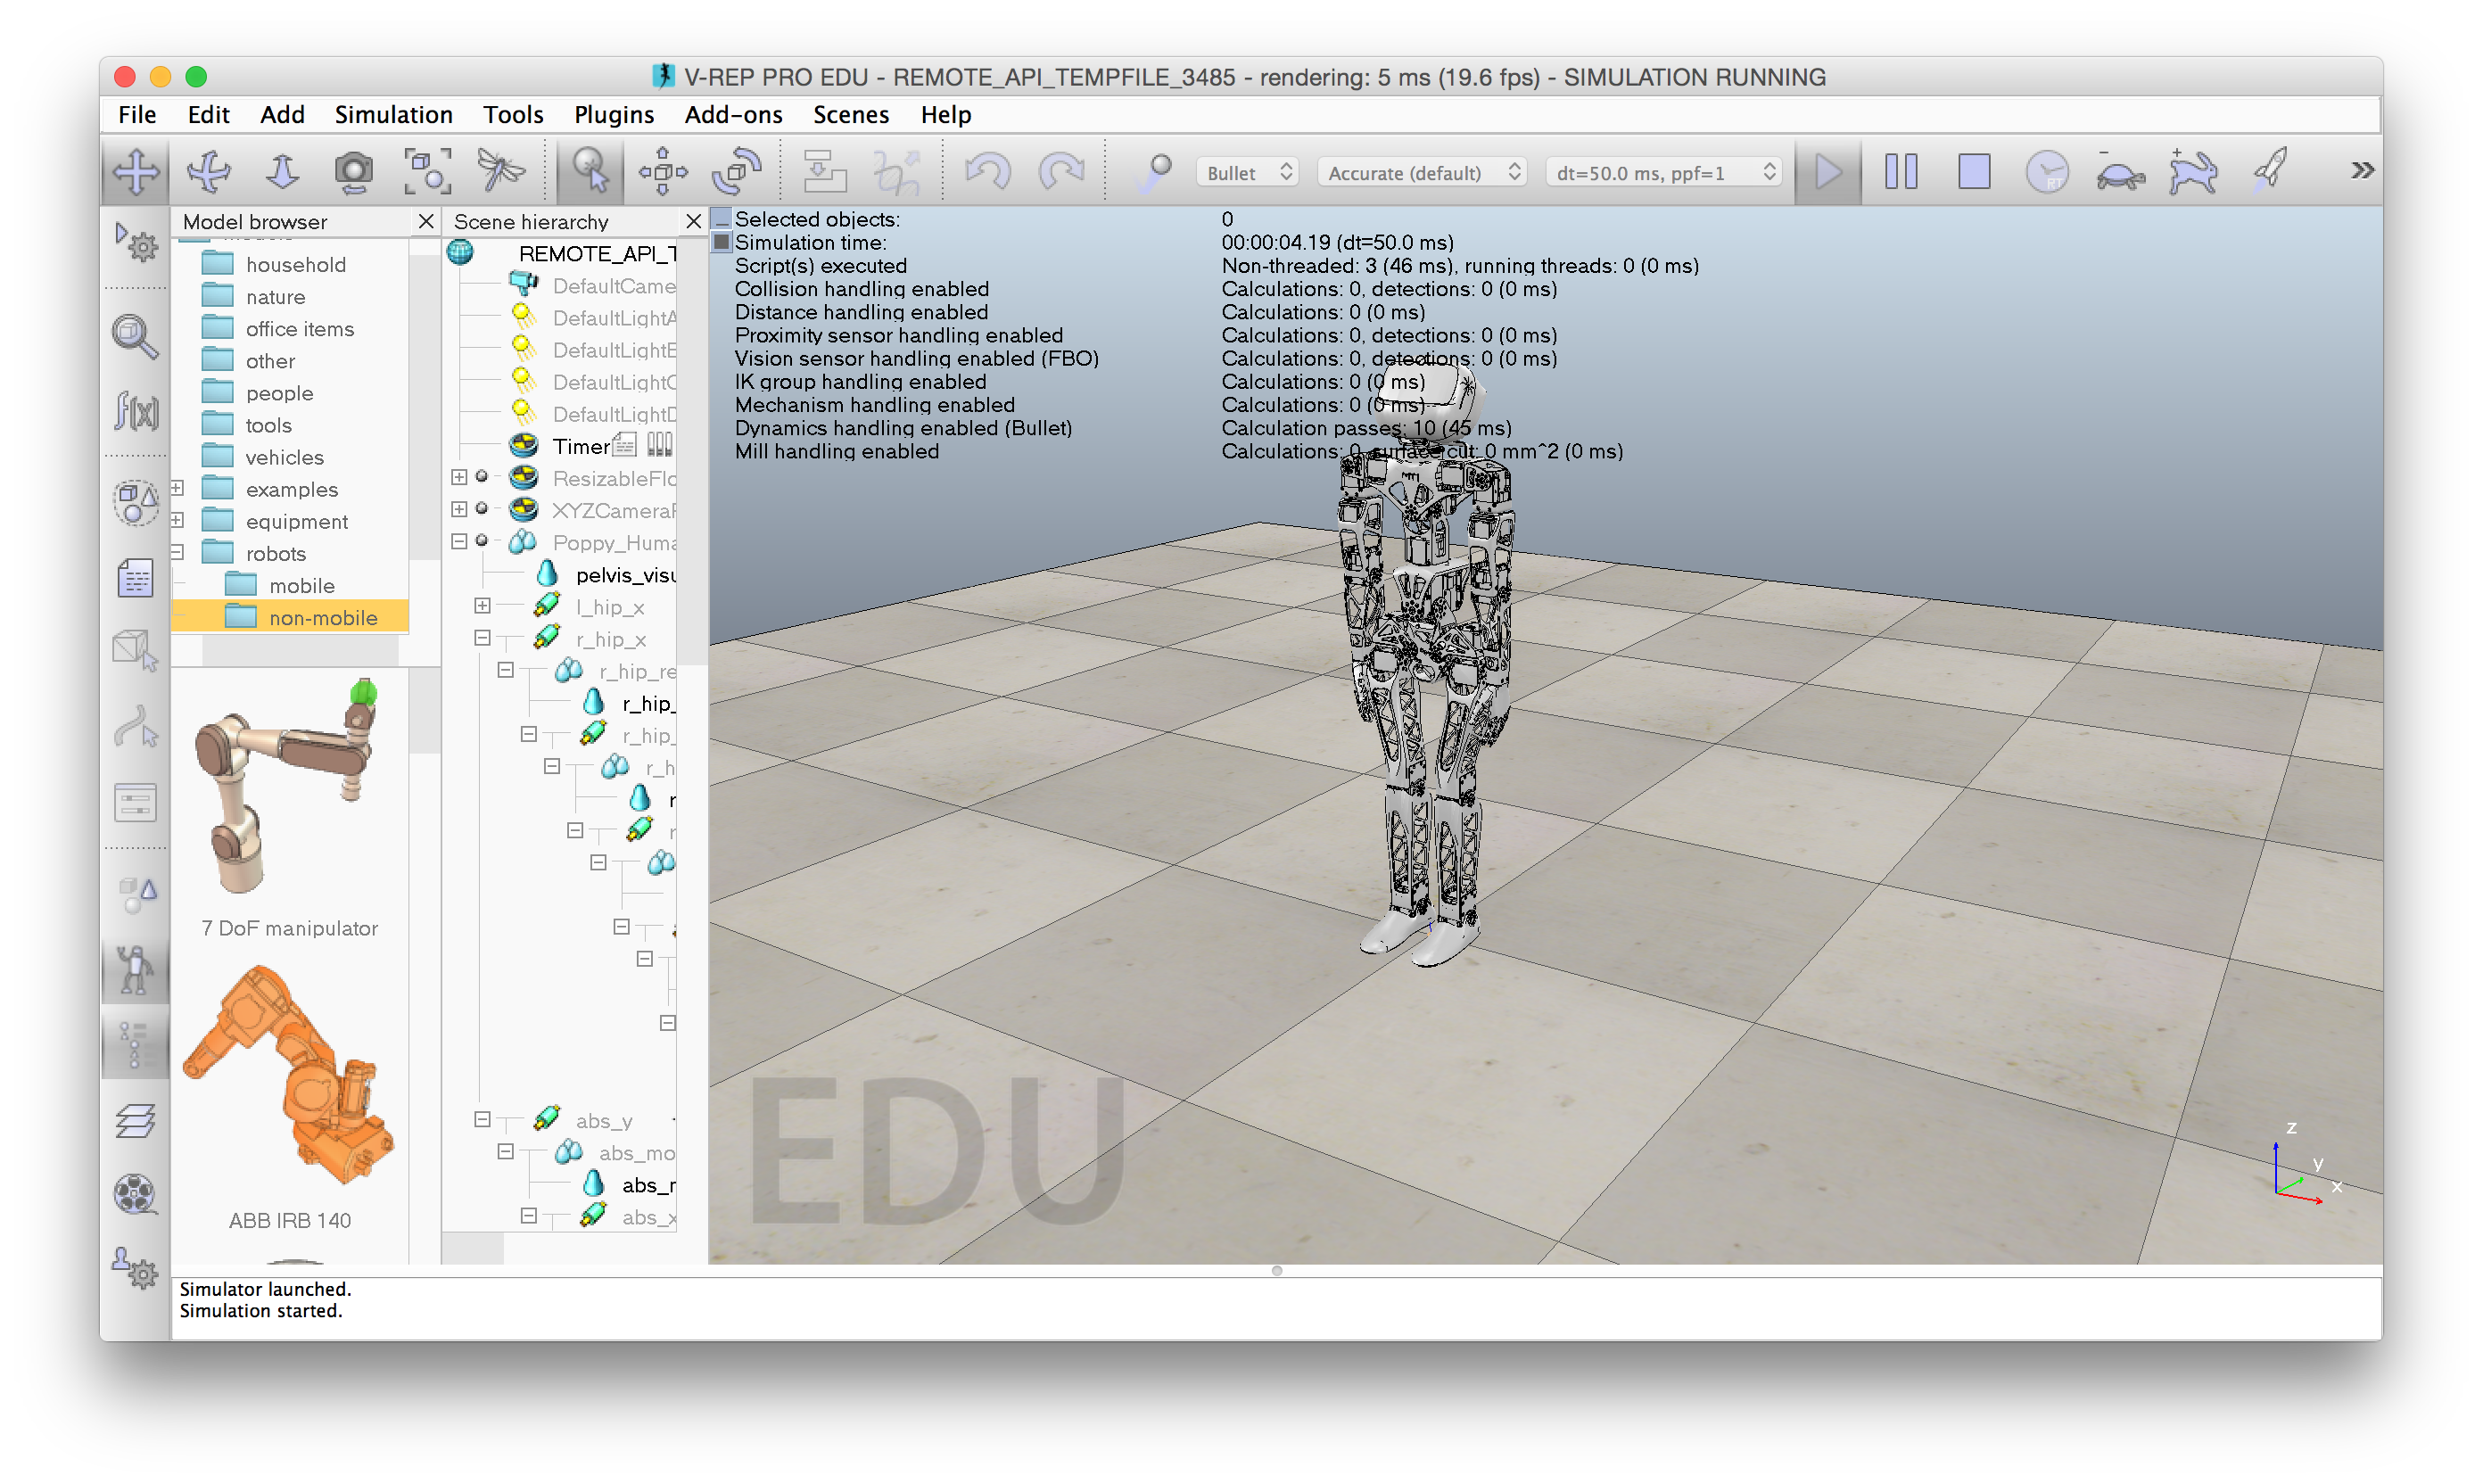
\includegraphics[width=0.8\textwidth]{img/vrep-poppy}
 \end{center}
   
Now you can control the simulated Poppy robot as a real robot, as presented in section \ref{pypot}.



\section{Visual programming with snap!}
\label{programming-with-snap}

\subsection{What is snap?}

\href{http://snap.berkeley.edu/}{Snap!} is a "very powerful visual, drag-and-drop programming language. It is an extended reimplementation of Scratch (a project of the Lifelong Kindergarten Group at the MIT Media Lab) that allows you to Build Your Own Blocks". It is an extremely efficient tool to learn how to program for kids or even college students and also a powerful prototyping method for artists.

 \begin{center}
  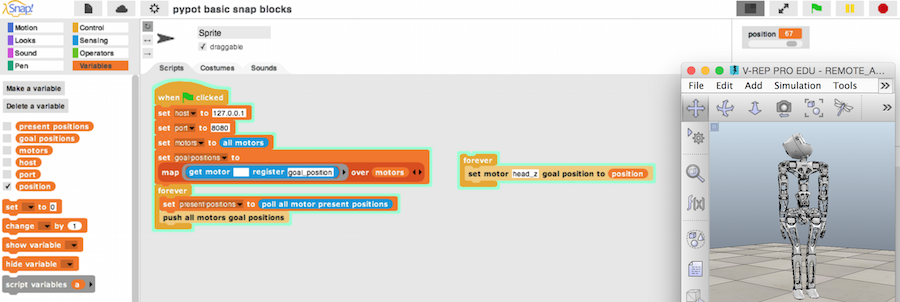
\includegraphics[width=0.9\textwidth]{img/snap-header}
 \end{center}

Snap! is open-source and it is entirely written in javascript, you only need a browser connected to the Poppy Creature webserver. No installation is required on your computer!

WARNING! As there is no browser installed by default in Poppy Humanoid's head, you can't use Snap! directly on the robot. You will have to connect the USB2AX to your computer or to use a simulated robot (see V-rep, section \ref{v-rep}).

\subsection{Creating the server}

The first step is to have a server running in the robot or in your computer. The Snap! page will then connect to this server to send orders to the robot.

\subsubsection{On a real Poppy Humanoid robot}

SSH inside the robot and enter the following command:

\begin{verbatim}
poppy-snap poppy-humanoid --no-browser
\end{verbatim}

This will create a PoppyHumanoid object and launch a snap server. It will also return a url (typically \url{http://snap.berkeley.edu/snapsource/snap.html#open:http://<IP>:6969/snap-blocks.xml}).

Enter this address in your web browser.

\subsubsection{On a simulated Poppy Humanoid robot}

For the v-rep simulator, open a Python console and enter:

\begin{verbatim}
from poppy_humanoid import PoppyHumanoid
poppy = PoppyHumanoid(simulator='vrep', use_snap=True)
poppy.snap.run()
\end{verbatim}

Then, open the following url in your web browser: \url{http://snap.berkeley.edu/snapsource/snap.html#open:http://127.0.0.1:6969/snap-blocks.xml}

\subsubsection{Running Snap! locally}

The previous paragraphes make you conect to the Berkeley server and use Snap! online. If you want to avoid this, you can \href{https://github.com/jmoenig/Snap--Build-Your-Own-Blocks}{install} Snap! locally.

Then, in your web browser, open the snap.html file. Import the Poppy specific blocks:

 \begin{center}
  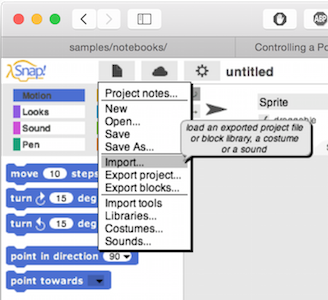
\includegraphics[width=0.6\textwidth]{img/snap-import}
 \end{center}

If you have Pypot installed from source, the file pypot-snap-blocks.xml is in the pypot/server folder. Otherwise, you can download only the file:
\begin{verbatim}
wget https://raw.githubusercontent.com/poppy-project/pypot/master/
pypot/server/pypot-snap-blocks.xml
\end{verbatim}

\subsection{Snap! quick start}

The webpage you opened should like like this:

 \begin{center}
  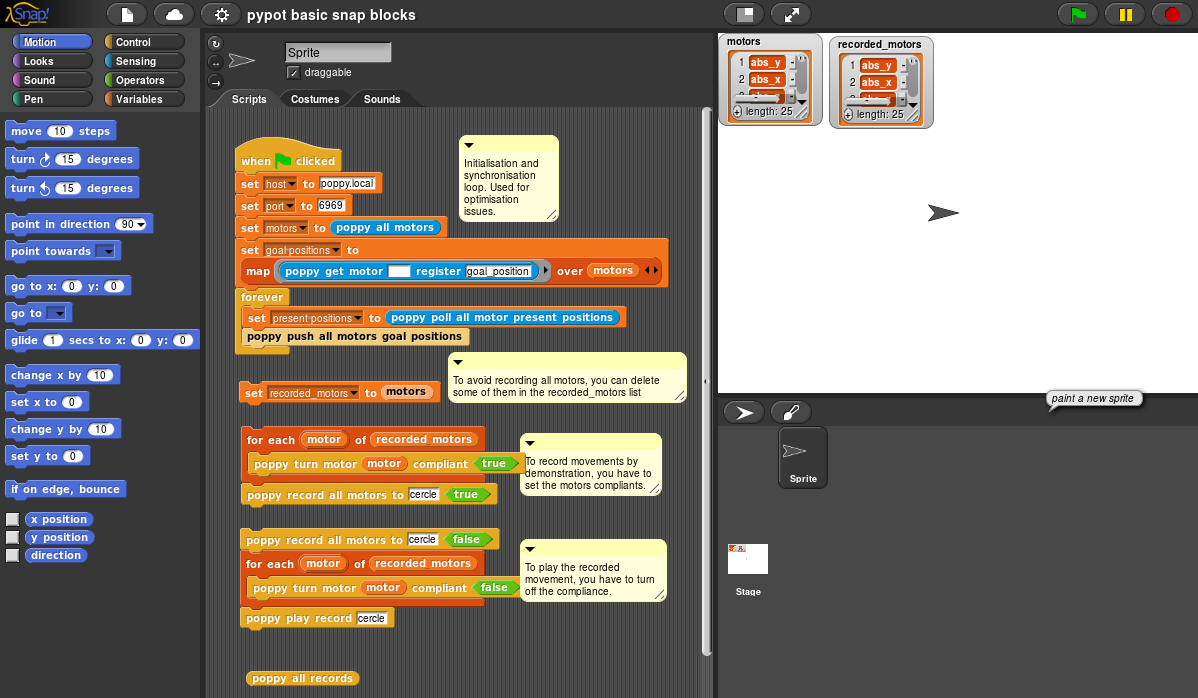
\includegraphics[width=0.8\textwidth]{img/snap_full}
 \end{center}

\subsubsection{Synchronization}

The first thing to do is to launch the synchronization loop. Replace the hostname by poppy.local if you use a real Poppy Humanoid robot. Then click on the loop, it should stay highlighted.

 \begin{center}
  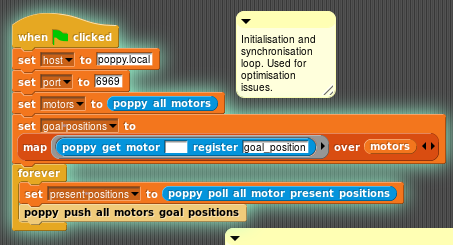
\includegraphics[width=0.8\textwidth]{img/snap_full_selected}
 \end{center}

This piece of code first set some variables: host, port, motors and goal-position, the later being created by reading the goal position  ('poppy get motor') of each motor present in the 'motors' array. You can check it by looking at the motors block top right:

 \begin{center}
  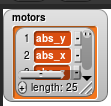
\includegraphics[width=0.3\textwidth]{img/snap_motors}
 \end{center}


Then we start a 'forever' loop that read the motors positions ('poppy poll all motors present positions') and store them in a present-positions array. Then it sends to the motors the content of the goal-position array.

This loop is the link between our Snap! code (we will read the present-positions array and modify the goal-positions array) and the real or simulated Poppy robot. You can stop the synchronization loop by clicking on it.

\subsubsection{Poppy blocks}

The default program shows you how to record a movement (called cercle by default):

 \begin{center}
  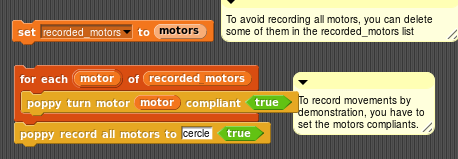
\includegraphics[width=0.8\textwidth]{img/snap_record}
 \end{center}
 
 The first line initializes an array containing all motors names. You need to run it only once.
 
 The next block turns all the motors to compliant, so you can move the robot by hand, and starts recording.
 
 To stop recording, click on the next block:
 
 
 \begin{center}
  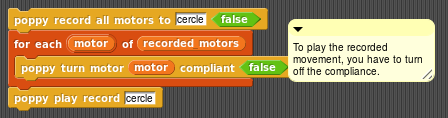
\includegraphics[width=0.8\textwidth]{img/snap_move}
 \end{center}
 
 This block stops the recording, then removes the compliance so that the robot can move by itself. Then, it starts playing the move you just recorded.
 
 \textbf{Warning}, if you record a move with a name that has already been used, the new movement will be added after the previous one! This may lead to unexpected movements from the robot. Moves are recorded as .record files in the home folder of the Poppy robot.
 
 Other Poppy specific blocks allow you to command each motor separately:
 
  \begin{center}
  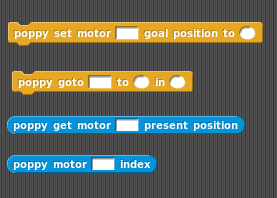
\includegraphics[width=0.6\textwidth]{img/snap_blocks}
 \end{center}

For other blocks, see the \href{http://snap.berkeley.edu/SnapManual.pdf}{Snap! reference manual}.


\section{The Pypot library for Poppy}
\label{pypot}

Pypot is a framework developed in the Inria FLOWERS team to make it easy and fast to control custom robots based on Dynamixel motors. This framework provides different level of abstraction corresponding to different types of use, i.e. direct control Robotis motors through a USB2AX, or high-level command of a robot defined by its particular structure.

Pypot has been entirely written in Python to allow for fast development, easy deployment and quick scripting by non-necessary expert developers. The serial communication is handled through the standard library and thus allows for rather high performance (10ms sensorimotor loop). It is crossed-platform and has been tested on Linux, Windows and Mac OS. It is distributed under the GPL V3 open source license.

Pypot is also compatible with the V-REP simulator. This allows you to seamlessly switch from a real robot to its simulated equivalent without having to modify your code.

Documentation can be found \href{http://poppy-project.github.io/pypot/index.html}{here}. %We do only a quick introduction here, find more in the advanced part, section \ref{•}.

\subsection{PoppyHumanoid}

%Use the ipython webservice (when ready) or 
Open a Python console inside the head of your PoppyHumanoid:

\begin{verbatim}
python
\end{verbatim}

The first step to control a Poppy robot with Pypot is to create a Python object corresponding to your robot. We call this object poppy and define it as a PoppyHumanoid:

\begin{verbatim}
from poppy_humanoid import PoppyHumanoid
poppy = PoppyHumanoid()
\end{verbatim}

This PoppyHumanoid object contains a list of motor objects that you can list with:

\begin{verbatim}
print poppy.motors
\end{verbatim}

You get something like:

\begin{verbatim}
[<DxlMotor name=l_elbow_y id=44 pos=-0.0>,
 <DxlMotor name=r_elbow_y id=54 pos=-0.0>,
 <DxlMotor name=r_knee_y id=24 pos=0.2>,
 <DxlMotor name=head_y id=37 pos=-22.7>,
 <DxlMotor name=head_z id=36 pos=0.0>,
 ...
\end{verbatim}

Each motor contain several fields, some static, like name and other directly linked to the corresponding Dynamixel register:

\begin{verbatim}
for m in poppy.motors:
  print "motor ",m.name
  print "  compliance: ",m.compliant,", position: ",m.present_position
\end{verbatim}

You end up with:

\begin{verbatim}
motor  abs_y
  compliance:  True , position:  45.14
motor  abs_x
  compliance:  True , position:  -21.41
motor  abs_z
  compliance:  True , position:  24.22
...
\end{verbatim}

Remember that the angular values are in degrees. When all motors are set to 0, the robot is standing with arms along the body.

You can also control each motor directly:

\begin{verbatim}
print "right ankle angle: ",poppy.r_ankle_y.present_position
\end{verbatim}

\subsection{Simple motor control}

To control a motor, you first need to allow it to use its torque, i.e. to stop being compliant. Let test on the left-right head motor (head\_z).

\begin{verbatim}
poppy.head_z.compliant = False
\end{verbatim}

To prevent the robot from being dangerous, we will limit its maximum torque. You will be able to slightly push the motor with your hand, but it will go back to its goal position. Max torque is an integer value between 0 and 100, a proportion of the physical motor max torque (depends on the motor model).

\begin{verbatim}
poppy.head_z.max_torque=20
\end{verbatim}

Then you have to set the goal position of the register. This operation is instantaneous and the servomotor will try to reach this position using a PID controller. But this is so quick that you will likely not see any delay.

\begin{verbatim}
poppy.head_z.goal_position=20
\end{verbatim}

 The communication with the Dynamixels itself takes some time and is done in parallel. So if you're using Python script, you need to add a bit of delay before the end, as the end of the script destroys you Poppy creature.
 
 \begin{verbatim}
import time
time.sleep(0.1)
\end{verbatim}

\subsection{Timed movements}

If you want a slower movement for your Dynamixel servomotor, you can use the goto\_position function and setting a time for the movement. 

\begin{verbatim}
poppy.head_z.goto_position(-20, 3)
\end{verbatim}

The head should go to angle -20 in 3 seconds.

The wait optional argument allows you to decide if you want the script to return immediately or to wait for the movement completion:

\begin{verbatim}
print "before moving"
poppy.head_z.goto_position(40, 3, wait=True)
print "after first movement completion"
poppy.head_z.goto_position(-40, 3, wait=False)
print "during second movement"
\end{verbatim}




%
%\section{Advanced guide}
%
%
%\subsection{Creating your own Poppy creature}
%\label{creating-poppy-creature}
%
%\subsection{Creating a primitive}
%
%\subsection{Quick look on Dynamixel registers}
%\label{dynamixel-registers}

%use code from others

%anaconda ?

%ipython notebooks ?

\section{Useful links}
\label{documentation-links}

\subsection{Forum and documentations}

\begin{tabular}{lr}

Poppy project website: & \url{https://www.poppy-project.org/} \\ 

Poppy project forum: & \url{https://forum.poppy-project.org/} \\ 
 
Pypot documentation: & \url{http://poppy-project.github.io/pypot/} \\ 

Github: & \url{https://github.com/poppy-project} \\ 

v-rep resources: & \url{http://www.coppeliarobotics.com/resources.html} \\ 
\end{tabular} 

\subsection{Other tutorials}

Poppy in V-REP:

\begin{flushright}
 \href{https://forum.poppy-project.org/t/howto-connect-pypot-to-your-simulated-version-of-a-poppy-humanoid-in-v-rep/332}{https://forum.poppy-project.org/t/howto-connect-pypot-\\to-your-simulated-version-of-a-poppy-humanoid-in-v-rep/332}
 \end{flushright}

Poppy and Snap!:

\begin{flushright}
\href{http://nbviewer.ipython.org/github/poppy-project/pypot/blob/master/samples/notebooks/Controlling%20a%20Poppy%20Creature%20using%20SNAP.ipynb}{http://nbviewer.ipython.org/github/poppy-project/pypot/blob/master/samples/notebooks/Controlling\%20\\a\%20Poppy\%20Creature\%20using\%20SNAP.ipynb}

\end{flushright}

Introduction to Pypot:
\begin{flushright}
\href{http://nbviewer.ipython.org/github/poppy-project/pypot/blob/master/samples/notebooks/QuickStart%20playing%20with%20a%20PoppyErgo.ipynb}{http://nbviewer.ipython.org/github/poppy-project/pypot/blob/master/samples/notebooks/\\QuickStart\%20playing\%20with\%20a\%20PoppyErgo.ipynb} 
\end{flushright}

Record and save moves:
\begin{flushright}
\href{http://nbviewer.ipython.org/github/poppy-project/pypot/blob/master/samples/notebooks/Record%2C%20Save%2C%20and%20Play%20Moves%20on%20a%20Poppy%20Creature.ipynb}{http://nbviewer.ipython.org/github/poppy-project/pypot/blob/master/samples/notebooks/\\Record\%2C\%20Save\%2C\%20and\%20Play\%20Moves\%20\\on\%20a\%20Poppy\%20Creature.ipynb} 
\end{flushright}

\end{document}
